\subsection{Android Application Package (APK)} \label{subsection:foundation-android-package}
\begin{itemize}
  \item uses apks from stores, downloaded oder developed
  \item zip format
  \item build process
  \item written in java, similar to java build  process, java compiler, obfuscator, packed to jar file
  \item java byte code to dalvik byte code, described later, obfuscation
  \item three main parts, classes.dex, resources, manifest, combined to archive file
  \item signing
  \item structure apk file
\end{itemize}

\begin{figure}[h]
    \centering
    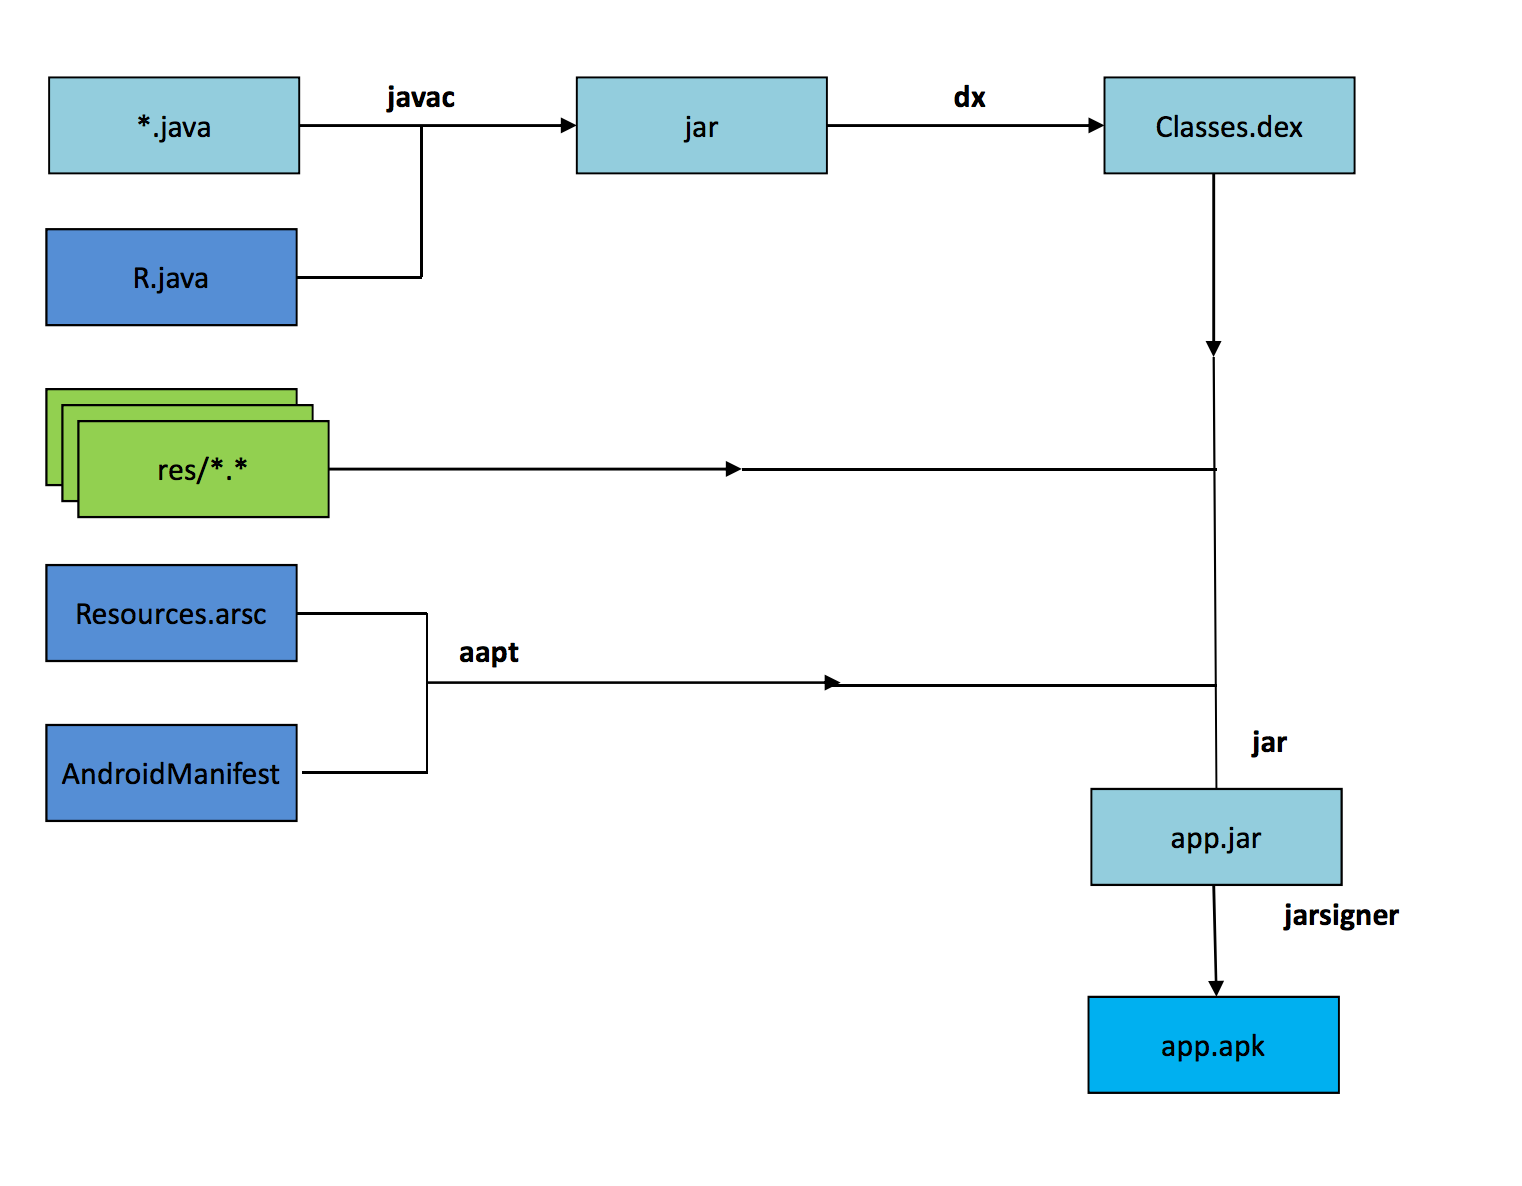
\includegraphics[width=0.8\textwidth]{data/apk.png}
    \caption{\gls{apk} build process \cite{andevconDalvikART}}
    \label{fig:apk}
\end{figure}
